\section{Introduction}

\begin{figure}[ht]
	\begin{center}
    	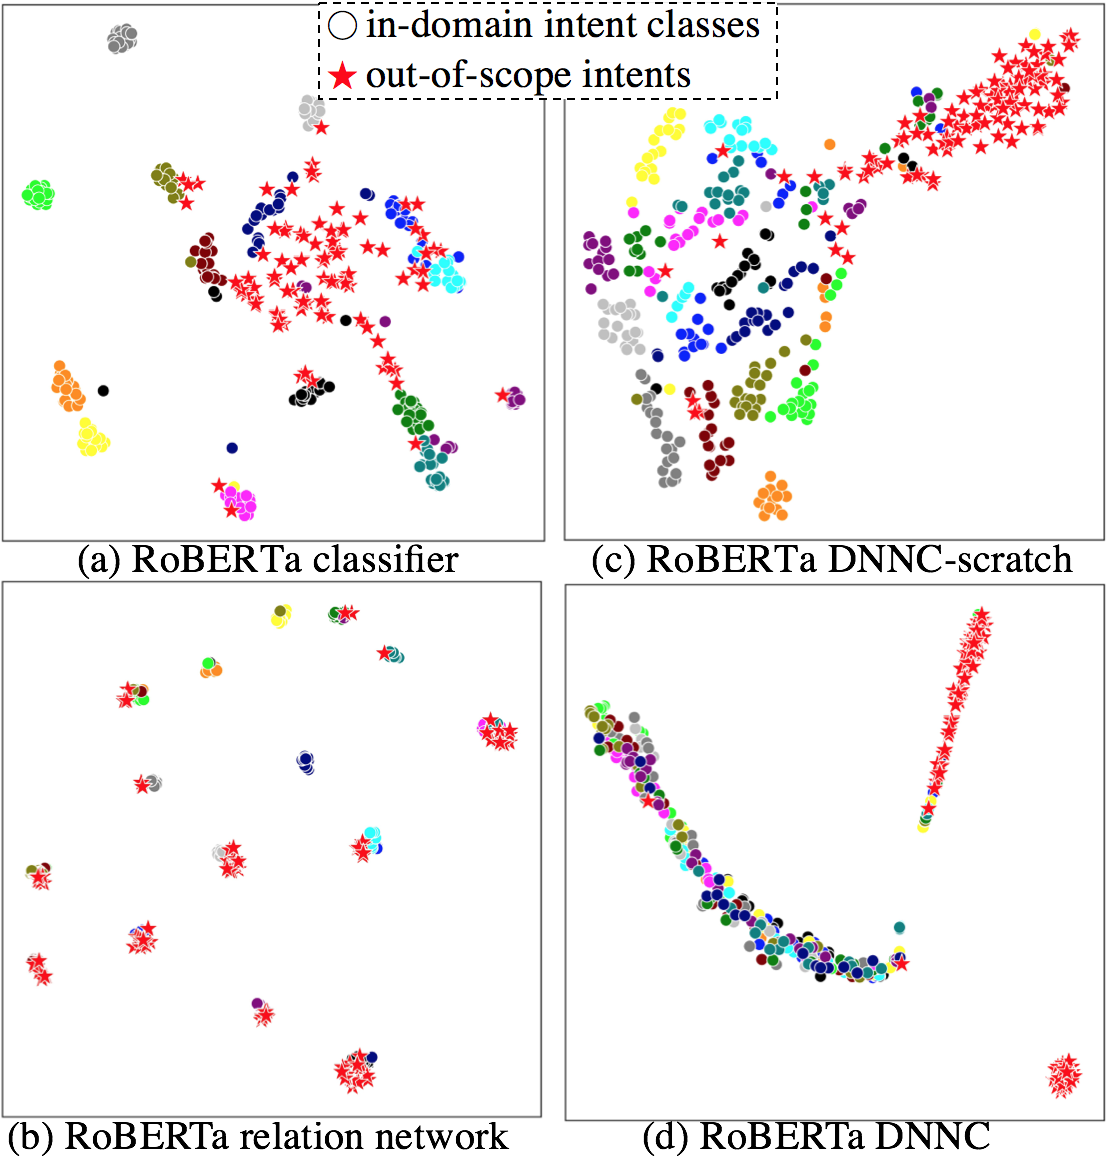
\includegraphics[width=1.0\linewidth]{./images/fig_tsne_main_more.png}
    \end{center}
% Interpretation/explanation by Wenhao
%\caption{Visual comparison for OOS detection between multi-class classifier and the proposed NLI-based approach, where encoded vectors for the [CLS] tokens are plotted using t-SNE.  Notice that the multi-class classifier is (mostly) successful in grouping examples from the same intent class close to each other, while create separation between in-domain and OOS samples for some classes. The proposed method, on the other hand, is able to create a near-perfect separation for OOS samples. Note that the proposed method \textbf{seeks to model a binary relationship between two utterances - whether the input and training examples belong to the same intent class or not}, instead of intent classes. This explains why in (b) the in-domain samples from different intents display no separation. }
\caption{tSNE visual comparison for OOS detection between existing methods ((a) and (b)) and our proposed method ((c) and (d)). Their embeddings before their classifier layers are used (best viewed in color).}
%\textcolor{red}{From Wenhao: let's rename the subfigures (c) and (d) to be consistent with our actual proposed methods names}}
% \textcolor{red}{Check: here is a hided Interpretation/explanation by Wenhao}
% The explanation will be addressed in the main body of Introduction.
\label{fig:tsne-main}
\vspace{-1em}
\end{figure}

Intent detection is one of the core components when building goal-oriented dialog systems.
%Although it has achieved a promising performance on some intent detection tasks~\cite{goo2018slot,xxxx}, it is still challengeable to accurately detect those user intents with few training examples due to the unconstrained user behaviour and growing domains.
The goal is to achieve high intent classification accuracy, and another important skill is to accurately detect unconstrained user intents that are out-of-scope (OOS) in a system~\citep{oos-intent}.
A practical challenge is data scarcity because different systems define different sets of intents, and thus few-shot learning is attracting much attention.
However, previous work has mainly focused on the few-shot intent classification without OOS~\citep{marrying-reg,efficient_intent}.
% mainly model the intent detection as a classification problem from the perspective of few-shot learning, without considering the out-of-scope (OOS) intents~\citep{marrying-reg,efficient_intent}.
% % mainly focus on few-shot intent classification without out-of-scope (OOS)~\citep{marrying-reg,efficient_intent}.

OOS detection can be considered as out-of-distribution detection~\citep{softmax_conf,learning_ood}.
Recent work has shown that large-scale pre-trained models like BERT~\citep{bert} and RoBERTa~\citep{roberta} still struggle with out-of-distribution detection, despite their strong in-domain performance~\citep{acl-ood}.
Figure~\ref{fig:tsne-main} (a) shows how unseen input text is mapped into a feature space, by a RoBERTa-based model for 15-way 5-shot intent classification.
The separation between OOS and some in-domain intents is not clear, which presumably hinders the model's OOS detection ability.
%Figure~\ref{fig:tsne-main} (b) further shows that this issue would not be easily mitigated even with more training examples.
This observation calls for investigation into more sample-efficient approaches to handling the in-domain and OOS examples accurately.

In this paper, we tackle the task from a different angle, and propose a discriminative nearest neighbor classification (DNNC) model.
Instead of expecting the text encoders to be generalized enough to discriminate both the in-domain and OOS examples, we make full use of the limited training examples both in training and inference time as a nearest neighbor classification schema.
We leverage the BERT-style paired text encoding with deep self-attention to directly model relations between pairs of user utterances.
We then train a matching model as a pairwise binary classifier to estimate whether an input utterance belongs to the same class of a paired example.
We expect this to free the model from having the OOS separation issue in Figure~\ref{fig:tsne-main} (a) by avoiding explicit modeling of the intent classes.
Unlike an embedding-based matching function as in relation networks~\citep{relation_net} (Figure~\ref{fig:tsne-main} (b)), the deep pairwise matching function produces clear separation between the in-domain and OOS examples (Figure~\ref{fig:tsne-main} (c)).
We further propose to seamlessly transfer a natural language inference (NLI) model to enhance this clear separation (Figure~\ref{fig:tsne-main} (d)).

We verify our hypothesis by conducting extensive experiments on a large-scale multi-domain intent detection task with OOS~\citep{oos-intent} in various few-shot learning settings.
Our experimental results show that, compared with RoBERTa classifiers and embedding nearest neighbor approaches, our DNNC attains more stable and accurate performance both in in-domain and OOS accuracy.
Moreover, our 10-shot model can perform competitively with a 50-shot or even full-shot classifier, with the performance boost by the NLI transfer.
We also show how to speedup our DNNC's inference time without sacrificing accuracy.
%\footnote{Our code is available at \url{https://github.com/salesforce/}.}
